\begin{frame}{Results --- Macroscopic validation}
    \begin{center}
    \resizebox{!}{0.25\textwidth}{
    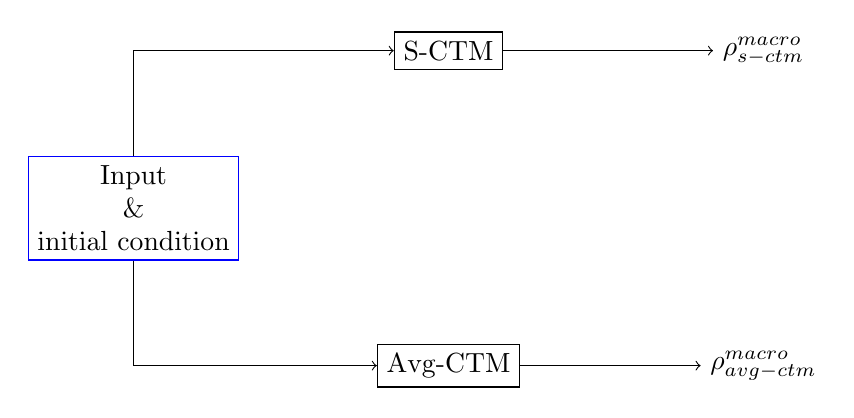
\begin{tikzpicture}
    \node[draw=blue, align=center] (input) at (0,0) {Input \\ \& \\ initial condition};
    \node[draw=black] (sctm) at (4,2) {S-CTM};
    \node[draw=black] (avgctm) at (4,-2) {Avg-CTM};
    \node (s) at (8,2) {$\rho^\text{macro}_\text{s-ctm}$};
    \node (avg) at (8,-2) {$\rho^\text{macro}_\text{avg-ctm}$};
    \draw[->] (input)|-(sctm);
    \draw[->] (input)|-(avgctm);
    \draw[->] (sctm)--(s);
    \draw[->] (avgctm)--(avg);
    \end{tikzpicture}
    }
    \end{center}
    \begin{center}
        \includegraphics[scale=0.45]{fig_55_validationSCTM}%
        \quad%\hspace{1em}%
        \includegraphics[scale=0.45]{fig_56_validationAvgCTM}%
    \end{center}
\end{frame}
